\documentclass[a4paper,12pt]{article}



\usepackage{graphicx}

\title{How to build a 4V geodesic dome}
\author{Andr\'{e} Franz}
\date{}


\begin{document}
\maketitle

For the 4V geodesic dome six different types of triangles are needed (Figure \ref{fig:triangles}). There are 30 triangles of each type needed, except for type 6 only 10 triangles are needed, see Table \ref{tab:amountoftriangles}.

\begin{figure}
	\centering
	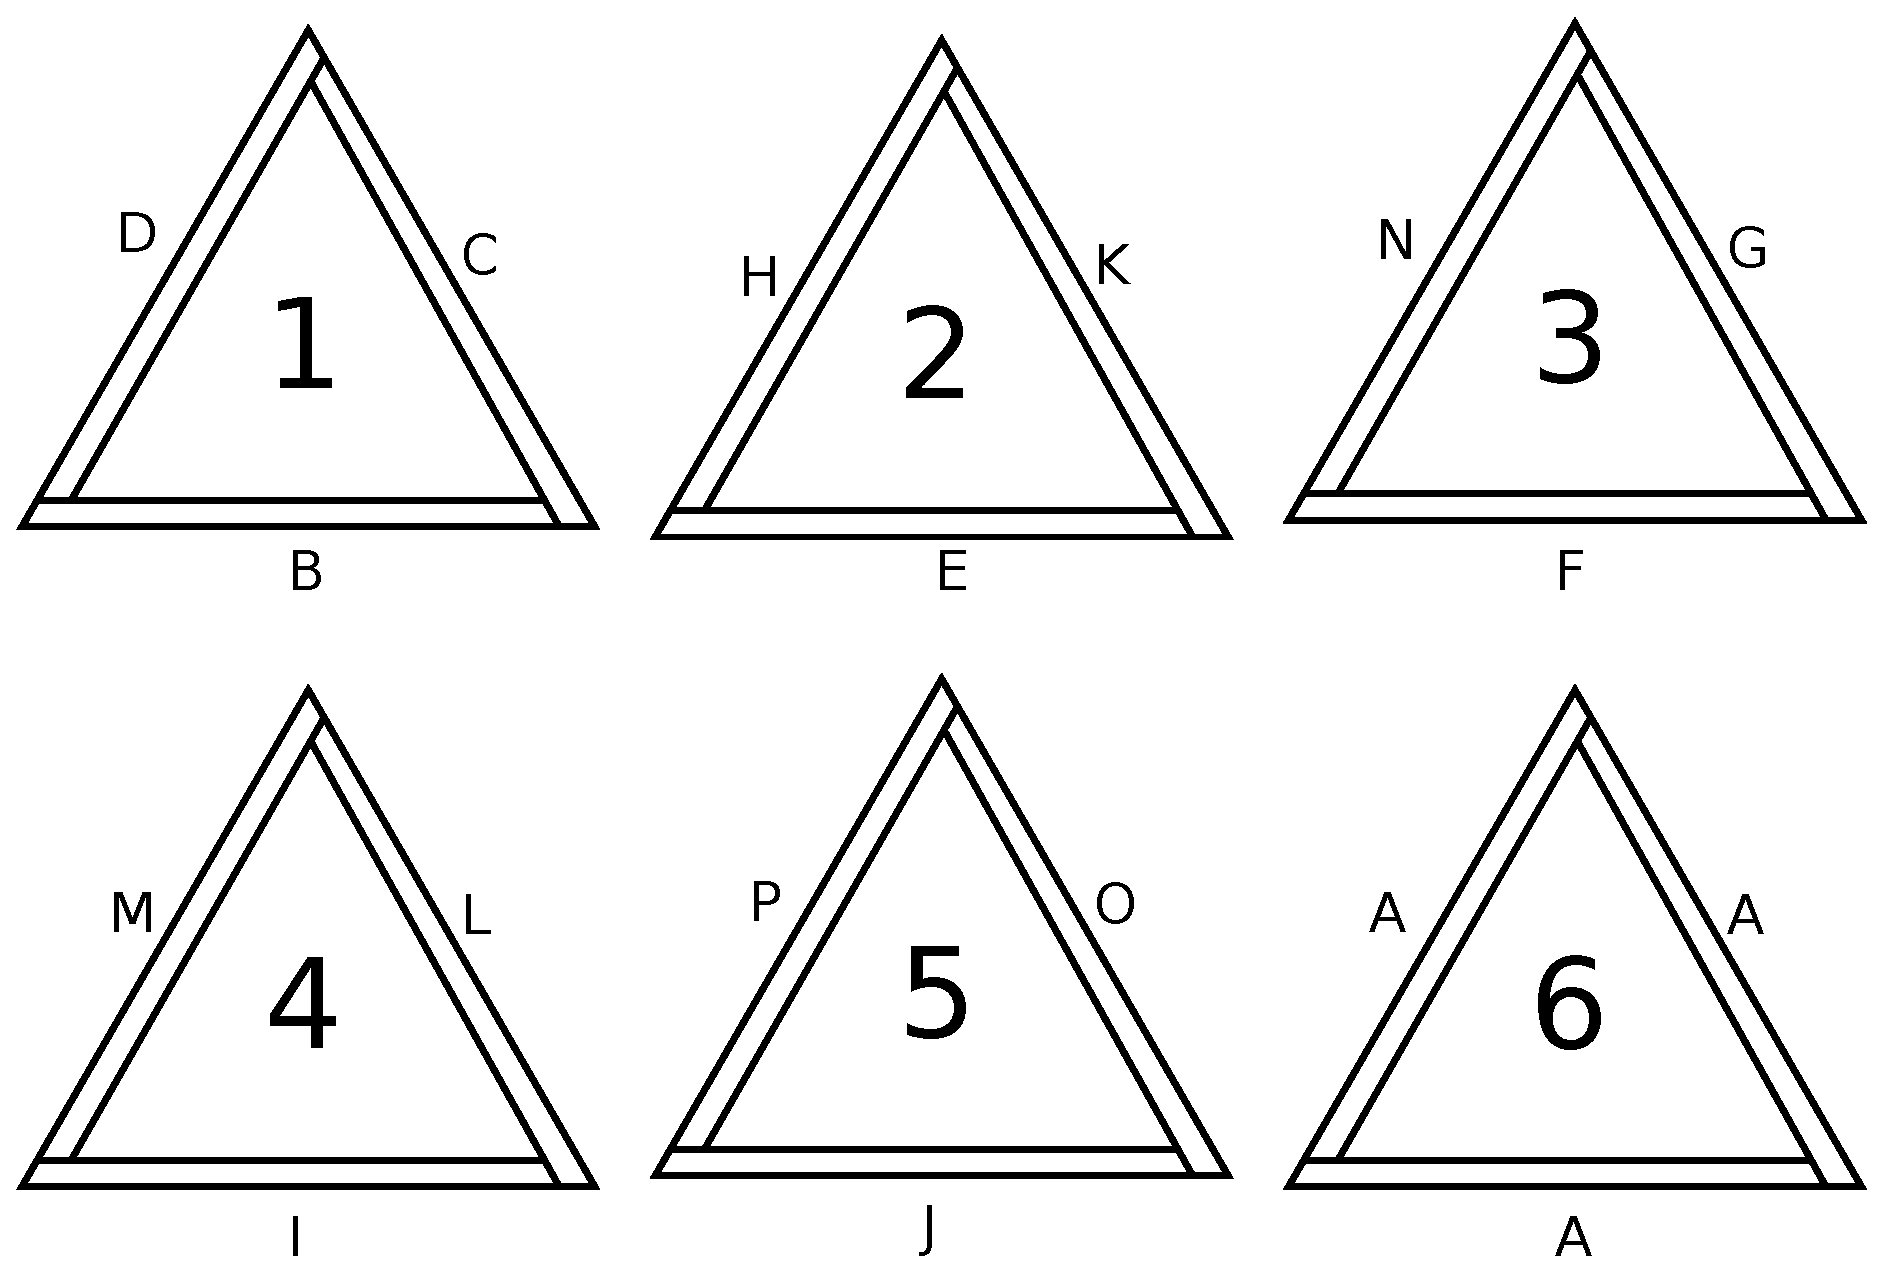
\includegraphics[width=\linewidth]{../images/4v_triangles.eps}
	\caption{Six different triangles are needed.}
	\label{fig:triangles}
\end{figure}


\begin{table}
	\centering
	\caption{Needed Amount of each triangle.}
	\begin{tabular}{l|llllll}
		Triangle type	& 1		& 2		& 3		& 4		& 5		& 6	\\ \hline
		Amount			& 30	& 30	& 30	& 30	& 30	& 10
	\end{tabular}
\label{tab:amountoftriangles}
\end{table}

\begin{table}
	\begin{tabular}{l|lll}
			& L			& L-l	& l		\\	\hline
		A	& 324.9 cm	&		&		\\
		B	& 324.9 cm	&		&		\\
		C	& 312.8 cm	&		&		\\
		D	& 312.8 cm	&		&		\\
		E	& 312.8 cm	&	&	\\
		F	& 312.8 cm	&	&	\\
		G	& 298.5 cm	&	&	\\
		H	& 298.5 cm	&	&	\\
		I	& 295.2 cm 	&	&	\\
		J	& 295.2 cm	&	&	\\
		K	& 294.5 cm	&	&	\\
		L	& 294.5 cm	&	&	\\
		M	& 294.5 cm	&	&	\\
		N	& 294.5 cm	&	&	\\
		O	& 253.1 cm	&	&	\\
		P	& 253.1 cm	&	&	
	\end{tabular}
\end{table}

\end{document}
